\documentclass[prd,tightenlines,preprintnumbers,showpacs,superscriptaddress,notitlepage,nofootinbib,eqsecnum,floatfix,notitlepage]{revtex4-1}

\usepackage{graphicx}
\usepackage{amsmath}
\usepackage{braket}
\usepackage{subcaption}
\usepackage{tikz}
\usepackage{float}
\usepackage[utf8]{inputenc} % supports umlaut natively, eg
%\usepackage[T1]{fontenc} 
\usepackage{hyperref} % adds hyperlinks
\usepackage{csvsimple} % Easily add csv file as table
\usepackage{booktabs} % For pretty tables
\usepackage{siunitx} % For rounding in tables
\usepackage{datatool}
\usepackage{url}
\usepackage{multirow}

\newcount\hour \newcount\hourminute \newcount\minute 
\hour=\time \divide \hour by 60
\hourminute=\hour \multiply \hourminute by 60
\minute=\time \advance \minute by -\hourminute
\newcommand{\mydate}{\ \today \ - \number\hour :\number\minute}


\begin{document}
	
\title{$F_K / F_\pi$ Notes}
\author{Nolan Miller}
\date{\mydate}


\begin{abstract}
In these notes, we explain our general fitting strategy for determining $F_K / F_\pi$. The description of the fit functions is mostly plagiarized from André's notes (though edited some for clarity), so kudos to him.
\end{abstract}
\maketitle

\subsection{Background}

\section{Fit Functions}

In general, our fits are of the form
\begin{equation}
\left(\frac{F_K}{F_\pi}\right)_\text{lattice} = \left(\frac{F_K}{F_\pi}\right)_\text{model}^{(n_V)} + 
\delta\left(\frac{F_K}{F_\pi}\right)_\text{NNLO} + 
\delta\left(\frac{F_K}{F_\pi}\right)_\text{NNNLO}
\end{equation}
where the $n_V$ denotes to which order we fit the finite volume effects.
\subsection{Special Functions}
For reference, we use the following special functions in our fits, which encapsulate the finite volume dependence. The values for the $c_n$'s are given in Table \ref{tab:cN_weights}.
\begin{align}
\mathcal{I}(m) &= \frac{m^2}{(4\pi)^2} \ln \left( \frac{m^2}{\mu^2} \right)
+ \frac{m^2}{4\pi^2} \sum_{|\mathbf{n}|\neq0} \frac{c_n}{mL|\mathbf{n}|} K_1(mL|\mathbf{n}|) \\
%%%
d\mathcal{I}(m) &=
\frac{1}{(4\pi)^2} + \frac{\mathcal{I}(m)}{m^2}
+\sum_{|\mathbf{n}|\neq0} \frac{c_n}{(4\pi)^2} \left[
\frac{2K_1(mL|\mathbf{n}|)}{mL|\mathbf{n}|}
-K_0(mL|\mathbf{n}|)
-K_2(mL|\mathbf{n}|)\right] \\
%%%
\mathcal{K}(m,M) &= \frac{1}{M^2 - m^2} \Big[ \mathcal{I}(M) - \mathcal{I}(m) \Big] \\
%%%
\mathcal{K}_{21}(m,M) &=
\frac{1}{(M^2 - m^2)^2} \Big[ \mathcal{I}(M) - \mathcal{I}(m) \Big]
-\frac{1}{M^2 - m^2} d\mathcal{I}(m) \\
%%%
\mathcal{K}(m_1,m_2,m_3) &= \frac{1}{m_1^2 - m_2^2}\frac{1}{m_1^2-m_3^2} \mathcal{I}(m_1)
+\frac{1}{m_2^2 - m_1^2} \frac{1}{m_2^2 - m_3^2} \mathcal{I}(m_2)
\nonumber\\&\phantom{=}
+\frac{1}{m_3^2 - m_1^2} \frac{1}{m_3^2 - m_2^2} \mathcal{I}(m_3)
\end{align}

%%%%%%%%%%%%%%%%%%%%%%%%%
% cN table
\begin{table}
	\begin{ruledtabular}
		\begin{tabular}{c|cccccccccc}
			$|\mathbf{n}|$& 1 & $\sqrt{2}$& $\sqrt{3}$& $\sqrt{4}$& $\sqrt{5}$& $\sqrt{6}$& $\sqrt{7}$& $\sqrt{8}$& $\sqrt{9}$& $\sqrt{10}$\\
			\hline
			$c_n$& 6&12& 8& 6& 24& 24& 0& 12& 30& 24
		\end{tabular}
	\end{ruledtabular}
	\caption{\label{tab:cN_weights}
		Finite volume weight factors for the first few finite volume modes.
	}
\end{table}



\subsection{NLO chiral extrapolation formulae}

In these expressions, the $\eta$ meson mass can be approximated with the $SU(3)$ Gell-Mann--Okubo formula
\begin{equation}
m_\eta^2 = \frac{4}{3} m_K^2 - \frac{1}{3}m_\pi^2\, .
\end{equation}
The $X$ mass appearing in the MA formulae is
\begin{equation}
m_X^2 = m_\eta + a^2 \Delta_{\rm I}
\end{equation}
where $a^2 \Delta_{\rm I}$ is the taste-identity mass splitting which MILC has determined~\cite{Bazavov:2012xda}.

The mixed meson masses are given by
\begin{equation}
m_{val,sea}^2 = \frac{1}{2}m_{val,val}^2 + \frac{1}{2}m_{sea,sea,5}^2 + a^2 \Delta_{\rm Mix}
\simeq m_{val,val}^2 + a^2 \Delta_{\rm Mix}\, .
\end{equation}
For brevity, we label a quark $j$ for sea-up, $u$ for valence-up, $r$ for sea-strange, and $s$ for valence-strange.

Given the quark mass tuning we have done, at LO in MA EFT~\cite{Chen:2006wf}, all partial quenching parameters are given by the taste-identity splitting
\begin{equation}
\Delta_{rs}^2 = \Delta_{ju}^2 = a^2 \Delta_{\rm I}\, .
\end{equation}

We can plot the splitting over flavors and pion masses, and see how well this LO relation holds.  We will also fit using the full on-shell masses as they appear in the MA formula as well as use an average mixed-meson mass splitting, $a^2 \Delta_{\rm mix}$, averaged over the flavors and ensembles (possibly replace the average with extrapolation).





\subsection{Models}
In the following descriptions of the models, we make use of the definitions
\begin{equation}
\epsilon_\pi^2 = \frac{m_\pi^2}{\Lambda_\chi^2} \qquad
\epsilon_K^2 = \frac{m_K^2}{\Lambda_\chi^2} \qquad
\epsilon_a^2 = \frac{a^2}{16 \pi ^2\omega_0^2} \qquad
\end{equation}
where we set $\Lambda_\chi^2$ to $F_\pi^2$, $F_K^2$, or $F_\pi F_K$.

\subsubsection{NLO MA}
For these fits, we will do
\begin{equation}
\left(\frac{F_K}{F_\pi}\right)_\text{MA} = \frac{F_K^\text{nlo}}{F_\pi^\text{nlo}}
\end{equation}
where
\begin{align}
\frac{F_\pi^{\rm nlo}}{F_0} &= 1
- \frac{\mathcal{I}(m_{ju})}{F^2}
-\frac{\mathcal{I}(m_{ru})}{2F^2}
+4 \epsilon_\pi^2 (4\pi)^2 (L_4 + L_5)
+8 \epsilon_K^2 (4\pi)^2 L_4
\end{align}

\begin{align}
\frac{F_K^{\rm nlo}}{F_0} &= 1
-\frac{\mathcal{I}(m_{ju})}{2F^2}
+\frac{\mathcal{I}(m_\pi)}{8F^2}
-\frac{\mathcal{I}(m_{ru})}{4F^2}
-\frac{\mathcal{I}(m_{sj})}{2F^2}
-\frac{\mathcal{I}(m_{rs})}{4F^2}
+\frac{\mathcal{I}(m_{ss})}{4F^2}
-\frac{3\mathcal{I}(m_X)}{8F^2}
\nonumber\\&\phantom{=}
+4\epsilon_\pi^2 L_4 + 4\epsilon_K^2(L_5 + 2L_4)
\nonumber\\&\phantom{=}
+\Delta_{ju}^2 \left[ -\frac{d\mathcal{I}(m_\pi)}{8F^2} + \frac{\mathcal{K(}m_\pi,m_X)}{4F^2} \right]
-\Delta_{ju}^4 \frac{\mathcal{K}_{21}(m_\pi,m_X)}{24 F^2}
\nonumber\\&\phantom{=}
+\Delta_{ju}^2\Delta_{rs}^2 \left[ \frac{\mathcal{K}_{21}(m_{ss},m_X)}{12F^2}
- \frac{\mathcal{K}(m_\pi, m_{ss}, m_X)}{6F^2} \right]
\nonumber\\&\phantom{=}
+\Delta_{rs}^2 \left[
\frac{\mathcal{K}(m_{ss},m_X)}{4F^2} 
-\frac{\mathcal{K}_{21}(m_{ss},m_X) m_K^2}{6F^2}
+\frac{\mathcal{K}_{21}(m_{ss},m_X) m_\pi^2}{6F^2}
\right]
\end{align}


\subsubsection{NLO MA Taylor expanded ratio}
For these fits, 

\begin{align}\label{eq:fkfpi_ma}
\left(\frac{F_K}{F_\pi}\right)_\text{MA Taylor} &= 1
+\frac{\mathcal{I}(m_{ju})}{2F^2}
+\frac{\mathcal{I}(m_\pi)}{8F^2}
+\frac{\mathcal{I}(m_{ru})}{4F^2}
-\frac{\mathcal{I}(m_{sj})}{2F^2}
+\frac{\mathcal{I}(m_{ss})}{4F^2}
-\frac{\mathcal{I}(m_{rs})}{4F^2}
-\frac{3\mathcal{I}(m_X)}{8F^2}
\nonumber\\&\phantom{=}
+\Delta_{ju}^2 \left[ -\frac{d\mathcal{I}(m_\pi)}{8F^2} + \frac{\mathcal{K(}m_\pi,m_X)}{4F^2} \right]
-\Delta_{ju}^4 \frac{\mathcal{K}_{21}(m_\pi,m_X)}{24 F^2}
\nonumber\\&\phantom{=}
+\Delta_{ju}^2\Delta_{rs}^2 \left[ \frac{\mathcal{K}_{21}(m_{ss},m_X)}{12F^2}
-\frac{\mathcal{K}(m_\pi, m_{ss}, m_X)}{6F^2}
 \right]
\nonumber\\&\phantom{=}
+\Delta_{rs}^2 \left[
\frac{\mathcal{K}(m_{ss},m_X)}{4F^2} 
-\frac{\mathcal{K}_{21}(m_{ss},m_X) m_K^2}{6F^2}
+\frac{\mathcal{K}_{21}(m_{ss},m_X) m_\pi^2}{6F^2}
\right]
\nonumber\\&\phantom{=}
+ 4 (4\pi)^2 L_5 \frac{m_K^2 - m_\pi^2}{(4\pi F)^2}
\end{align}

\subsubsection{NLO $\chi$PT}
For these fits, we will do
\begin{equation}
\left(\frac{F_K}{F_\pi}\right)_\text{$\chi$PT} = \frac{F_K^{\rm nlo}}{F_\pi^{\rm nlo}}
\end{equation}
where
\begin{align}
\frac{F_\pi^{\rm nlo}}{F_0} &= 1
- \frac{\mathcal{I}(m_\pi)}{F^2}
-\frac{1}{2}\frac{\mathcal{I}(m_K)}{F^2}
+4 \epsilon_\pi^2 (4\pi)^2 (L_4 + L_5)
+8 \epsilon_K^2 (4\pi)^2 L_4 \, , \\
\frac{F_K^{\rm nlo}}{F_0} &= 1
-\frac{3}{8}\frac{\mathcal{I}(m_\pi)}{F^2}
-\frac{3}{4}\frac{\mathcal{I}(m_K)}{F^2}
-\frac{3\mathcal{I}(m_\eta)}{8F^2}
+4\epsilon_\pi^2 L_4 + 4\epsilon_K^2(L_5 + 2L_4)
\end{align}


\subsubsection{NLO $\chi$PT Taylor expansion}
For these fits, 
\begin{align}\label{eq:fkfpi_chpt}
\left(\frac{F_K}{F_\pi}\right)_\text{$\chi$PT Taylor} &= 1
+\frac{5}{8} \frac{\mathcal{I}(m_\pi)}{F^2}
-\frac{1}{4} \frac{\mathcal{I}(m_K)}{F^2}
-\frac{3}{8} \frac{\mathcal{I}(m_\eta)}{F^2}
%\nonumber\\&\phantom{=}
+4(\epsilon_K^2 - \epsilon_\pi^2) (4\pi)^2 L_5
%\nonumber\\&\phantom{=}
+ \delta_{c.t.}^{\rm NNLO}
\end{align}

\subsubsection{NLO MA Taylor (old)}
This fit was taken from (17) of \cite{Berkowitz:2017opd}. {\color{red} (To do: add to notes.)}




\subsection{Corrections}

\subsubsection{NNLO \& NNNLO counter terms}
The NNLO and NNNLO counter terms are formed by taking powers of $\epsilon^2_\xi$ ($\xi = K, \pi, a$), along with $(\epsilon_K^2 - \epsilon_\pi^2)$ (which ensures $F_K / F_\pi$ tends to 1 in the chiral limit), to the desired order. For NNLO, we take one power of $\epsilon^2_\xi$ and one power of $(\epsilon_K^2 - \epsilon_\pi^2)$. 
\begin{equation}
\delta\left(\frac{F_K}{F_\pi}\right)_\text{NNLO} = \bigg[ 
\epsilon_a^2  A_{a}
+\epsilon_K^2  A_{K}
+\epsilon_\pi^2  A_{\pi}
\bigg] (\epsilon_K^2 - \epsilon_\pi^2)
\end{equation}
One might expect a term like $(\epsilon_K^2 - \epsilon_\pi^2)^2 A_{\chi}$ to show up in the NNLO expansion; however, this term is already covered by $[\epsilon_K^2  A_{K}+\epsilon_\pi^2  A_{\pi}] (\epsilon_K^2 - \epsilon_\pi^2)$.

For NNNLO, we take two powers of $\epsilon^2_\xi$ and one power of $(\epsilon_K^2 - \epsilon_\pi^2)$ (and vice-versa).
\begin{align}
\delta\left(\frac{F_K}{F_\pi}\right)_\text{NNNLO} &= \bigg[
\epsilon_a^4  A_{a, a} + \epsilon_a^2 \epsilon_K^2  A_{a, K} + \epsilon_a^2 \epsilon_\pi^2  A_{a, \pi} \\ \nonumber
&\phantom{[ =} + \epsilon_K^4  A_{K, K} + \epsilon_K^2 \epsilon_\pi^2  A_{K, \pi} \\ \nonumber
&\phantom{[ =} + \epsilon_\pi^4  A_{\pi, \pi} \bigg] (\epsilon_K^2 - \epsilon_\pi^2)
\end{align}

Notice that the lattice spacing and $am_\xi$ ($\xi \in \{\pi, K, \eta\}$) corrections are included in these counterterms. For example, the term $\epsilon^2_a (\epsilon^2_K - \epsilon^2_\pi)$ accounts for the lowest order lattice spacing correction. Further note that our choice of action (Domain wall) means that the theory will automatically be $\mathcal{O}(a)$ improved~\cite{Berkowitz:2017opd}, hence the lack of terms at that order.

\subsubsection{ SU(2) isospin breaking}
The breaking of SU(2) isospin symmetry is characterized by
\begin{equation}
\delta_{\text{SU(2)}} = \sqrt{3} \epsilon_\text{SU(2)} \left[
-\frac43 (F_K / F_\pi-1)
+\frac{4}{3(4 \pi F)^2} \left( m_K^2 - m_\pi^2 -m_\pi^2 \log \frac{m_k^2}{m_\pi^2} \right)
\right]
\end{equation}
where $\epsilon_\text{SU(2)} = \sqrt{3}/(4R)$, $R=35.7(2.6)$ per FLAG, the masses are the physical values, and $F_K/F_\pi$ is the fitted value extrapolated to the physical point. With $\delta_{\text{SU(2)}}$ in hand, we can compare our value of $F_K/F_\pi$ determined on the lattice to the corrected charged ratio $F^\pm_K/F^\pm_\pi$ through
\begin{equation}
\frac{F^\pm_K}{F^\pm_\pi} = \frac{F_K}{F_\pi} \sqrt{1+ \delta_{\text{SU(2)}}} \, .
\end{equation}
The corrected charge ratio $F^\pm_K/F^\pm_\pi$ is the value reported by FLAG. 

%%%%%%%%%%%%%%%%%%
%%%%% FIT STRATEGY
%%%%%%%%%%%%%%%%%%
\section{Fit Strategy}

From inspections, one sees that the fit depends on the pion, kaon, and mixed meson masses; the taste-identity splitting $\Delta_{rs}^2 = \Delta_{ju}^2 = a^2 \Delta_\text{I}$; the lattice spacing $a$; the Wilson flow scale $w_0$; and the pion and kaon decay constants. First we briefly explain how these quantities were determined, then how we can use them to determine $F_K / F_\pi$ at the physical point.


\subsection{Meson masses}
The meson masses are determined by fitting the spectral decomposition of the meson two-point correlation functions.
\begin{equation}
C(t) = \sum_n Z^{(PS)}_{n} Z^{(SS)}_{n} \left( e^{-E_n t} + e^{-E(T-t)} \right)
\end{equation}

Usually it's sufficient to fit only a single exponential, so we only need to choose the start and end times for our fit. Further, by symmetrically fitting the interval $[t, T - t]$, we reduce these three fit choices to only one -- determining the start time.

Once the mass has been determined over the full ensemble (boot0), the correlation function is resampled $N$ times to form $N$ bootstrap resamples. These bootstrap resamples are then fit over the same time range as the full ensemble and the results are saved, giving us a list of masses for bootstrapping.

\subsection{Taste-identity splitting}
As previously stated, this quantity has been determined by MILC~\cite{Bazavov:2012xda}.

\subsection{Wilson flow scale $\omega_0$}
The Wilson flow-derived quantity $\omega_0$ allows for high-precision scale setting~\cite{Borsanyi:2012zs}. In general, one can measure the lattice spacing by comparing the lattice value of some (dimensionful) observable to its experimental value, eg, 
\begin{equation}
a = \frac{(a m_\Omega)^\text{latt}}{m_\Omega^\text{exp}}
\end{equation}
which can be converted to physical units by multiplying by $\hbar c$ (ie, $a_\text{phys} = a \hbar c$). Similarly, one can determine $\omega_0$ by measuring
\begin{equation}
w_0 = \frac{(w_0 m_\Omega)^\text{latt}}{m_\Omega^\text{exp}} \, , 
\end{equation}
a task currently underway in another project.  {\color{red} (Is this right?)} In particular, given the following observable
\begin{equation}
W(t) \equiv t \frac{d}{dt} \Big[ t^2 \langle E(t) \rangle \Big] \, ,
\end{equation}
the scale $w_0$ is the value such that 
\begin{equation}
W(t) \Big|_{t=w_0^2} = 0.3 \, .
\end{equation}

For the purpose of this project, we take $w_0 = 0.175(10)$, which is a conservative estimate taken from current progress on scale setting. 

\begin{figure}
	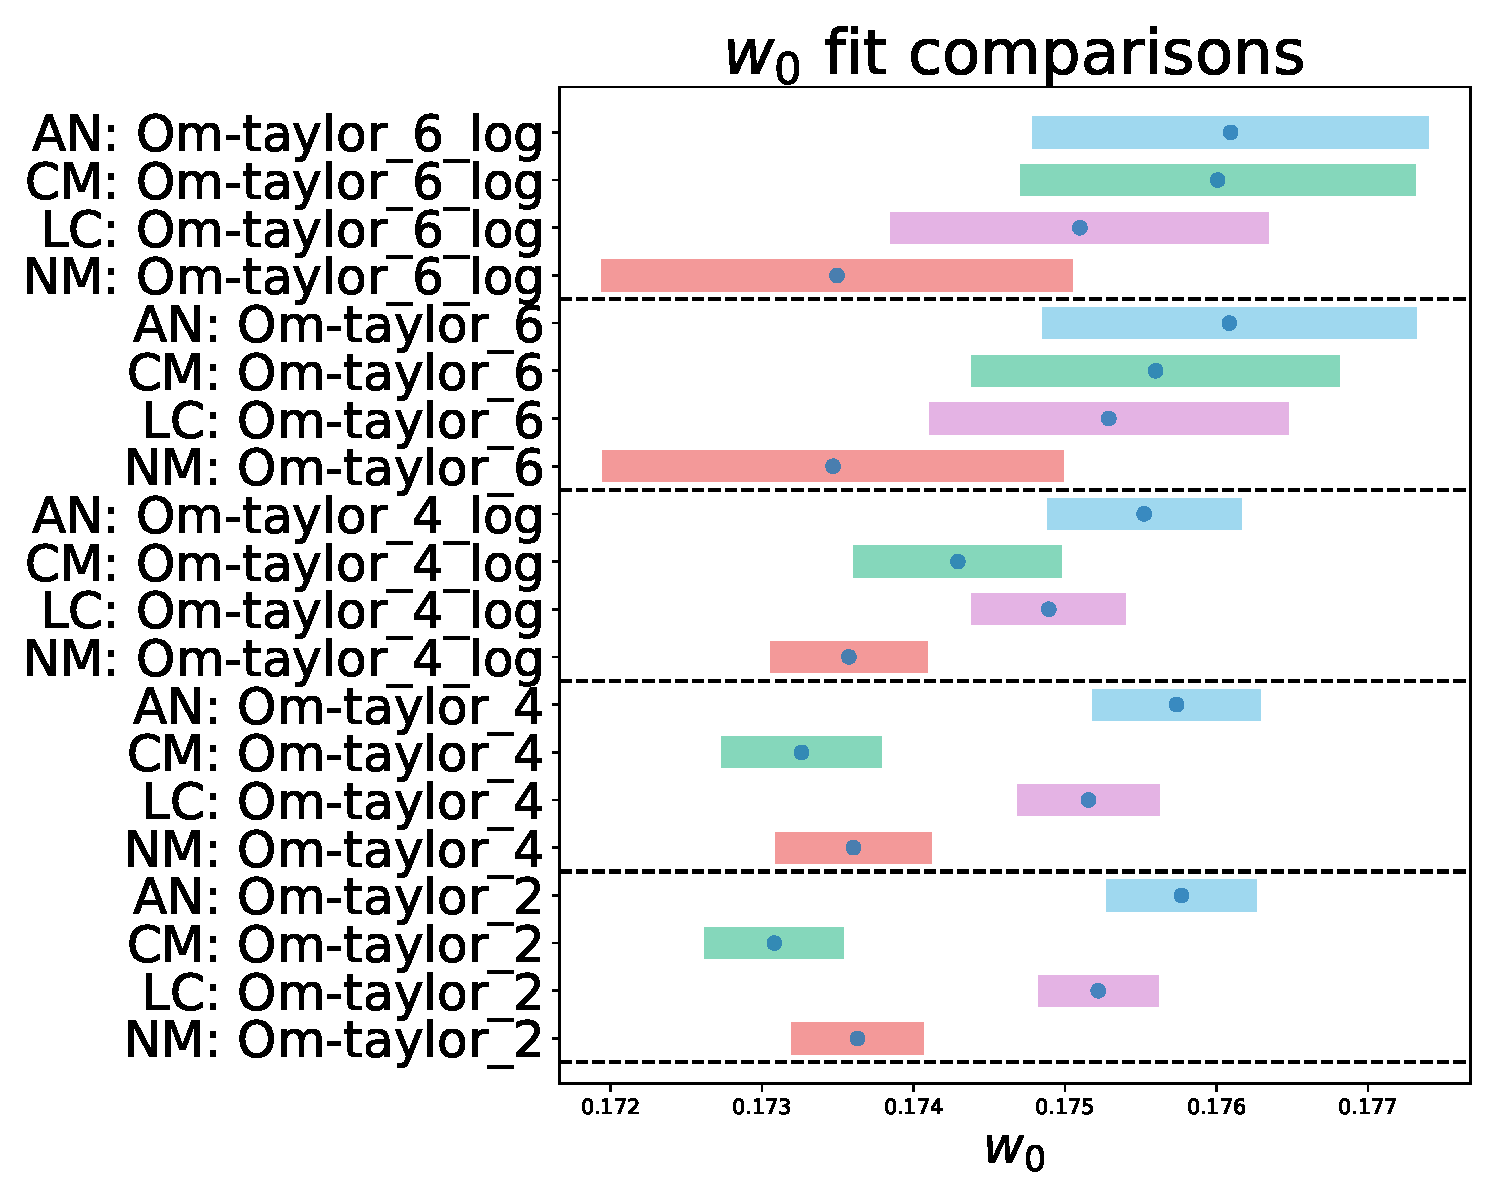
\includegraphics[width=0.75\textwidth]{./../figs/w0_comparison.pdf}
	\caption{Current results on scale setting. Notice that our conservative choice for $w_0$ contains all the models in the figure and then some.}
\end{figure}




\subsection{The pion and kaon decay constants, $F_K$ and $F_\pi$}
{\color{red} (How are these determined?)}






\section{The Weeds}
The actual fit here is performed in lattice units, not physical units, which is possible since the ratio $F_K / F\pi$ is dimensionless.

\subsection{Selection of Prior}

\begin{table}[]
	\begin{tabular}{l|llc}
		& LEC          & Term                                          & \begin{tabular}[c]{@{}l@{}}Order at \\ Phys Point\end{tabular} \\ \hline\hline
		\multirow{3}{*}{NNLO}  & $A_a$        & $\epsilon^2_a \epsilon^2_\chi$                & 0                                                              \\
		& $A_K$        & $\epsilon^2_K \epsilon^2_\chi$                & $\sim10^{-2}$                                                  \\
		& $A_\pi$      & $\epsilon^2_\pi \epsilon^2_\chi$              & $\sim10^{-3}$                                                  \\ \hline
		\multirow{6}{*}{NNNLO} & $A_{aa}$     & $\epsilon^4_a \epsilon^2_\chi$                & 0                                                              \\
		& $A_{a\pi}$   & $\epsilon^2_a \epsilon^2_\pi \epsilon^2_\chi$ & 0                                                              \\
		& $A_{aK}$     & $\epsilon^2_a \epsilon^2_K \epsilon^2_\chi$   & 0                                                              \\
		& $A_{KK}$     & $\epsilon^4_K \epsilon^2_\chi$                & $\sim 10^{-3}$                                                 \\
		& $A_{K\pi}$   & $\epsilon^2_K \epsilon^2_\pi \epsilon^2_\chi$ & $\sim 10^{-4}$                                                 \\
		& $A_{\pi\pi}$ & $\epsilon^2_K \epsilon^2_\pi \epsilon^2_\chi$ & $\sim 10^{-5}$                                                
	\end{tabular}
	\caption{Contributions from each LEC at the physical point. Here we define $\epsilon^2_\chi = (\epsilon^2_K -\epsilon^2_\pi)$, which ensures $F_K/F_\pi \rightarrow 1$ in the SU(3) isospin limit.}
\end{table}

\subsubsection{Current method}
\begin{enumerate}
	\item At NLO, the most naive guess is that the LECs $L_4$ and $L_5$ should be order 1. Running the fit a few times, we quickly discover that these LECs are a few orders of magnitude smaller. Therefore, refining our priors for $L_4$ and $L_5$, we set \texttt{p[`L\_4'] = 0(0.001)} and \texttt{p[`L\_5'] = 0(0.001)}. In practice this width extends about an order of magnitude outside our results for $L_4$ and $L_5$, regardless of NLO model chosen.
	
	\item For the next higher order (NNLO) fit, we chain the result of the previous (NLO) fit into the fitter. If $L\pm\sigma_L$ is the result for an NLO LEC as determined by the NLO fit (ie, $L_5$ or $L_4$), then for the NNLO fit we take the prior for the NLO LECs to be \texttt{p[`L']=L(3*$\sigma_L$)}.
	
	\item To determine the priors for the NNLO LECs, we use the empirical Bayes criterion, which is implemented in \texttt{lsqfit} through \texttt{lsqfit.empbayes\_fit}. In this process, we set all the NNLO LECs $A_\xi$ to have prior \texttt{p[`A$_\xi$'] = 0($\lambda$)}, and we allow $\lambda$ to vary until a fit is produced such that the logGBF is maximized.
\end{enumerate}

\subsubsection{Old Method}
Barring some good physical argument for the expected value of the priors, we use the following heuristic.
\begin{enumerate}
	\item At NLO, the most naive guess is that the LECs $L_4$ and $L_5$ should be order 1. Running the fit a few times, we quickly discover that these LECs are a few orders of magnitude smaller. Therefore, refining our priors for $L_4$ and $L_5$, we set \texttt{p[`L\_4'] = 0(0.001)} and \texttt{p[`L\_5'] = 0(0.001)}. In practice this width extends about an order of magnitude outside our results for $L_4$ and $L_5$, regardless of NLO model chosen.
	
	\item To set the NNLO priors, we first determine the order of magnitude of the $\epsilon^2_\xi (\epsilon^2_K - \epsilon^2_\pi)$ terms. For example, $\epsilon^2_a (\epsilon^2_K - \epsilon^2_\pi) \sim 10^{-3}$. We center our prior at 0, but set it wide enough such that the upper/lower ends of the uncertainty interval could produce an LEC $A_\xi$ st $\epsilon^2_\xi A_\xi  (\epsilon^2_K - \epsilon^2_\pi) \sim 10^{-2}$, which ensures that the prior doesn't exclude the LEC from contributing at the percent level. In the case of $ \epsilon^2_a (\epsilon^2_K - \epsilon^2_\pi)$, we would set \texttt{p[`A\_a'] = 0(10)}. The procedure is similar for the NNNLO LECs, with us again setting the priors st the LECs can potentially contribute at the percentile level.
\end{enumerate}
While this procedure potentially allows all the NNLO and NNNLO LECs to contribute to the fits, it does lead to some pretty absurd results when taken at face value; eg, setting \texttt{p[`A\_aa'] = 0(100000)}, as one would do as described above, results in a fit of $A_{a, a} = -4926 (11908)$. Fortunately, the \texttt{logGBF} of these fits are correspondingly penalized.

\subsection{Comparison of results for taylor expanded NLO models}
As a first test of our fits, André and I performed the \texttt{ma-taylor} and \texttt{xpt-taylor} fits at NLO on each ensemble, where there is only one parameter that needs to be determined ($L_5$). See fig \ref{fig:L5-comparison}.

\begin{figure}
	\begin{subfigure}[t]{0.45\textwidth}
		\includegraphics[width=\textwidth]{./../tmp/L5_comparison_ma-taylor.pdf}
	\end{subfigure}
	~
	\begin{subfigure}[t]{0.45\textwidth}
		\includegraphics[width=\textwidth]{./../tmp/L5_comparison_xpt-taylor.pdf}
	\end{subfigure}
	\caption{Value of $L_5$ as independently determined by me (NM) and André. The difference between the central values is likely caused by my choice to use \texttt{boot0} vs André's choice to use the mean of the bootstrap list. }
	\label{fig:L5-comparison}
\end{figure}

\subsection{Effect of NNLO LECs on fit convergence}
We compare the effect of adding each NNLO LEC to the fit as well as the effect of chaining the fits. The priors for the NNLO LECs were set in accordance to the method described earlier in these notes, unless the figure corresponds to not chaining the fits, in which case that step is skipped. 

\foreach \model in {ma, ma-taylor, xpt, xpt-taylor}
{
	\begin{figure}[H]
		\begin{subfigure}[t]{0.45\textwidth}
			\includegraphics[width=\textwidth]{"./../tmp/exclude_lecs/\model__chained-True__exclude-n2lo".pdf}
		\end{subfigure}
		~
		\begin{subfigure}[t]{0.45\textwidth}
			\includegraphics[width=\textwidth]{"./../tmp/exclude_lecs/\model__chained-False__exclude-n2lo".pdf}
		\end{subfigure}
	\caption{Effect of individually including NNLO LECs for model \texttt{\model}. The topmost (non-FLAG) result is equivalent to the NLO fit; the bottommost is equivalent to the NNLO fit. See table \ref{\model-prior} for prior.}
	\end{figure}
}

\subsection{Shifting lattice data to physical point}
Notice that the fit of $F_K/F_\pi$ depends on multiple input parameters: $\epsilon^2_\pi$, $w_0$, $a$, etc; that is, we are fitting a many-dimensional surface, so in order to plot $F_k/F_\pi$ vs some parameter, we must carefully take a slice of that surface. In our case, we fit $F_K / F_\pi$ at the physical point with the exception of some input parameters, which we allow to vary.  

Of course, our set of data is not at the physical point, so we must account for this when making these plots. We therefore ``shift" the lattice data to the physical point (while allowing a single parameter to vary) using the following heuristic. Let $\{p_j\} = \{\epsilon^2_\pi, w_0, a, \cdots\}$ be the set of input parameters in the fit for some ensemble and $\{p^*_j\}$ the physical value of these parameters. Now suppose we are interested in the dependence of $F_K / F_\pi$ on some subset of the parameters $\{q_k\}$. Then to shift the data to the physical point without shifting $\{q_k\}$, we calculate
\begin{equation}
\left( \frac{F_K}{F_\pi} \right)_\text{shifted data} =
\left( \frac{F_K}{F_\pi} \right)_\text{data}
+ \left( \frac{F_K}{F_\pi} \right) \bigg|_{\text{fit at } \{p^*_j, q_k\}}
- \left( \frac{F_K}{F_\pi} \right) \bigg|_{\text{fit at } \{p_j, q_k\}} \, .
\end{equation}

Alternatively, one often uses the ratio instead.

\begin{equation}
\left( \frac{F_K}{F_\pi} \right)_\text{shifted data} =
\left( \frac{F_K}{F_\pi} \right)_\text{data}
\Bigg[ \left( \frac{F_K}{F_\pi} \right) \bigg|_{\text{fit at } \{p^*_j, q_k\}}
\bigg/ \left( \frac{F_K}{F_\pi} \right) \bigg|_{\text{fit at } \{p_j, q_k\}} \, \Bigg] .
\end{equation}

I haven't noticed a visible difference in using one versus the other.


\section{Fit Results}
Here we present the results for each of the fits.

\begin{figure}
	\includegraphics[width=0.9\textwidth]{./../tmp/fit_comparison.pdf}
	\caption{Extrapolations of $F^\pm_K/F^\pm_\pi$ to the physical point for the various models, with the FLAG result shown as a red band.}
\end{figure}

\begin{figure}
	\includegraphics[width=0.9\textwidth]{./../tmp/delta-su2_comparison.pdf}
	\caption{Extrapolations of $\delta_{\text{SU(2)}}$ to the physical point for the various models.}
\end{figure}

%\csvautotabular[respect all]{"./../results/fit"_"results".csv}
%\begin{tabular}{|l|c|}%\hline%
%	\sisetup{round-mode=places, round-precision=3}
%	fit & logGBF \\ \hline\hline
%	\csvreader[head to column names]%
%	{"./../results/fit_results".csv}{}%
%	{\\ \fit & \num{\logGBF}}%
%	\\\hline
%\end{tabular}


\DTLloaddb{myDB}{"./../results/fit_results".csv}

% Convoluted function used to escape underscore
\DeclareUrlCommand\UScore{\urlstyle{rm}}
\newcommand{\expUScore}{%
	\expandafter\expandafter\expandafter
	\UScore
	\expandafter\expandafter\expandafter
}

% Table for fit results
\begin{table}
\begin{center}
	\sisetup{round-mode=places,
		table-number-alignment = center-decimal-marker
	}
	\begin{tabular}{l|lllll}\toprule
		\textbf{Name} & $F^\pm_K/F^\pm_\pi$ & $\delta_{\text{SU(2)}}$ & logGBF & $Q$ & $\chi^2_\nu$%
		\DTLforeach*{myDB}{\Name=name, \Fit=fit, \delta=delta_su2, \logGBF=logGBF, \Q=Q, \chi=chi2/df}{%
			\DTLiffirstrow{\\\hline\\}{\\}%
			\expUScore{\Name} & \Fit & \delta &\num{\logGBF} & \num{\Q} & \num{\chi}
		}%
		\\\bottomrule
	\end{tabular}

\end{center}
\caption{Results of models and statistics}
\end{table}

% Table for LEC results
\begin{table}
	\begin{center}
		\sisetup{round-mode=places,
			table-number-alignment = center-decimal-marker
		}
		\begin{tabular}{l|ll|lll|llllll}\toprule
			\textbf{Name} & $L_5$ & $L_4$ & $A_a$ & $A_\pi$ & $A_K$ & $A_{aa}$ & $A_{a\pi}$ & $A_{aK}$ & $A_{KK}$ & $A_{K\pi}$ & $A_{\pi\pi}$ %
			\DTLforeach*{myDB}{\Name=name, \Lfive=L_5, \Lfour=L_4, \Aa=A_a, \Ap=A_p, \Ak=A_k, \Aaa=A_aa, \Aap=A_ap, \Aak=A_ak, \Akk=A_kk, \Akp=A_kp, \App=A_pp}{%
				\DTLiffirstrow{\\\hline\\}{\\}%
				\expUScore{\Name} & \Lfive & \Lfour & \Aa & \Ap & \Ak & \Aaa & \Aap & \Aak & \Akk & \Akp & \App
			}%
			\\\bottomrule
		\end{tabular}
		
	\end{center}
	\caption{Determined LECs}
\end{table}

% Tables for priors
\begin{table}
\foreach \model in {ma, ma-taylor, xpt, xpt-taylor}
{
	\begin{minipage}{0.20\textwidth}
		\begin{tabular}{l|l}
			\textbf{LEC} & \textbf{Value}
			\DTLloaddb[noheader,keys={lec,value},headers={lec,value},omitlines=1]{\model-prior-db}{"./../priors/\model".csv}
			\DTLforeach*{\model-prior-db}{\lec=lec, \value=value}{%
				\DTLiffirstrow{\\\hline\\}{\\}%
				\texttt{p[`\expUScore{\lec}']} & \value
			}%
		\end{tabular}
		\caption{\texttt{\model}}
		\label{\model-prior}
	\end{minipage}
	\hspace*{-0.01\textwidth}
}
\end{table}


% Plot fits vs eps2_pi
\foreach \model in {ma, ma-taylor, xpt, xpt-taylor}
{
	\subsection{\tt \model}
	\foreach \order in {nlo, nnlo, nnnlo}
	{
		\begin{figure}[H]
			\caption{\model (\order)}
			\includegraphics[width=\textwidth, page=3]{"./../tmp/fits/\model"_"\order".pdf}
		\end{figure}
	}
}

\appendix
\section{Physical Point Values}
The physical point values are given in Table \ref{table:phys_point_values}. The pion and kaon masses are taken from \cite{Berkowitz:2017opd} while the mass for the $\eta^\prime = (ss)$ meson is taken from \cite{Dowdall:2013rya}; however, we could have just as readily taken $m_{ss}^2 = 2 m_K^2 - m_\pi^2$ evaluated at the physical point (see Fig \ref{fig:mss}).

\begin{figure}
	\includegraphics[width=0.9\textwidth]{./../tmp/mss_vs_mk_mpi.pdf}
	\caption{Comparison of $m_{ss}^2$ and $2m_K^2 - m_\pi^2$.}
	\label{fig:mss}
\end{figure}

\begin{table}[]
	\begin{ruledtabular}
		\begin{tabular}{lll||lll||lll}
		$a/w_0$ & $L$      & $a^2 \Delta_I$ & $m_\pi$ (MeV)   & $m_K$ (MeV)     & $m_{ss}$ (MeV)   & $F_\pi$ (MeV)   & $F_K$ (MeV)      & $F_K^\pm/F_\pi^\pm$ \\
		\hline\
		0       & $\infty$ & 0              & $134.8(3)$ & $494.2(3)$& $688.5(2.2)$ & $91.9(3.5)$ & $110.38(64)$ & $1.1932(19)$       \\
		\end{tabular}	
	\end{ruledtabular}
\caption{Values used when extrapolating to the physical point; $F_K^\pm/F_\pi^\pm$ is taken from FLAG (and is not used for the extrapolation).}
\label{table:phys_point_values}
\end{table}

\bibliography{notes}

\end{document}

